% !TEX ROOT = ../ersti.tex
\section{EDV}

\subsection{Universitätsrechenzentrum (URZ)}
\label{urz}
Computer sind die Triebfeder unseres Zeitalters und auch im Studium kommt ihr nicht um sie herum. Das beginnt zum Beispiel schon damit, dass die meisten Übungszettel nur online erscheinen und selbst ausgedruckt werden müssen. Später möchtet ihr eure Bachelor- oder Masterarbeit bzw.\ eure Examensarbeit sicher nicht handschriftlich anfertigen sondern lieber in \LaTeX \footnote{„Latech“ gesprochen. OpenOffice -- oder noch schlimmer -- Word helfen nicht weiter, weil man Formeln nur sehr umständlich eingeben kann. Außerdem schafft es \LaTeX{} Blocktexte ohne größere Freiräume und mit weniger Bindestrichen zu setzen, wie man z.\,B.\ an diesem Ersti-Info sehen kann. Wenn ihr \LaTeX{} lernen möchtet, haltet in den nächsten Semestern nach einem entsprechenden Kurs Ausschau oder nutzt eins der vielen Onlinetutorials.} setzen. Das  \gls{URZ} bietet eine ganze Menge von Services an, die hier kurz erläutert werden sollen.

\subsection*{Multifunktionaler Studierendenausweis (Campus Card)}
\label{campuscard}
Wie an den meisten Unis ist der Studierendenausweis auch in Heidelberg voll modern und also multifunktional.
Neben der Ausweisfunktion wird er zum Ausleihen von Büchern in der Universitätsbibliothek und als „Geldkarte“ zum Bezahlen sowohl in der Mensa als auch an Kopierern benutzt. Um diese Funktion nutzen zu können, muss man Geld auf den Ausweis laden, dafür stehen in den Mensen Automaten zur Verfügung.
Zusätzlich gilt der Ausweis im \gls{VRN} werktags ab 19 Uhr und an Wochenenden ohne Zeitbegrenzung auch als Fahrausweis (siehe auch \autopageref{verkehrsmittel}).

Auf dem RFID-Chip der Karte ist nur die ID für die Bezahlfunktion des Studentenwerks gespeichert und daher auch die einzige Information, die sich ohne Sichtverbindung auslesen lässt. Sofern euer Geldbeutel dünn genug ist und die Campus Card nicht durch Kleingeld, Bankkarten o.ä. abgeschirmt wird, lässt sich sogar durch auflegen des Geldbeutel bezahlen -- allerdings sind die Lesegeräte nicht besonders stark und auch nicht besonders schnell, sodass ihr das am besten dann ausprobiert, wenn nicht so viel Betrieb ist. Alle anderen Informationen wie euer Name, die Matrikelnummer usw. sind lediglich aufgedruckt.
.
Wichtig ist vor allem, dass euer Studierendenausweis auch validiert ist, sonst ist er nämlich nicht gültig. Diese Validierung müsst ihr jedes Semester nach eurer Rückmeldung durchführen, vergesst das nicht!

\subsection*{Account}
Damit ihr überhaupt Zugang zum URZ bekommt, benötigt ihr Nutzername
und Passwort. Euer Nutzername („Uni-ID“) ist auf eurem multifunktionalen Studentenausweis aufgedruckt.
Um dann den Account nutzen zu können, muss die Uni-ID auf der Seite \url{http://freischalten.uni-hd.de} freigeschaltet werden. Hier könnt ihr auch euer Passwort und eure Uni-E-Mail-Adresse auswählen.
Die Freischaltung kann man auch direkt beim Infoservice im URZ erledigen.

\subsection*{E-Mail}
Mit der Freischaltung erhaltet ihr automatisch eine E-Mail-Adresse die auf \emph{@stud.uni-heidelberg.de} endet und mit momentan 200 MB Speicherplatz nicht so schlecht ausgestattet ist. Größter Vorteil ist ihre Werbefreiheit und sehr gute Verfügbarkeit. \textbf{Achtung:} Solltet ihr die Adresse trotz allem nicht verwenden wollen, ändert \emph{unbedingt} eure Stammdaten im LSF\footnote{\url{https://lsf.uni-heidelberg.de}}. Viele wichtige E-Mails wie die Rückmelde"=Erinnerung, Nachrichten von euren TutorInnen oder Rundmails der Vorlesungen gehen dort ein.

\sidebar{
    \centering{
        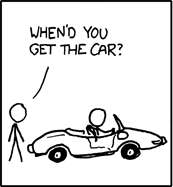
\includegraphics[width=3cm]{bilder/new_car_1.png}\\\vspace{20mm}
        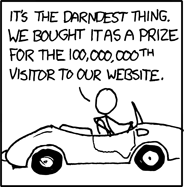
\includegraphics[width=3cm]{bilder/new_car_2.png}\\\vspace{20mm}
        
\includegraphics[width=3cm]{bilder/new_car_3.png}\\\vspace{20mm}
        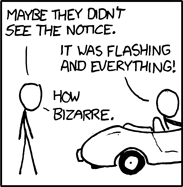
\includegraphics[width=3cm]{bilder/new_car_4.png}
    }
}

\subsection*{Drucken}

Zum Drucken kann man seine Dokumente auf einen speziellen Druck-Server\footnote{\url{http://drucker.uni-hd.de}} laden und dann an (fast) jedem der über den Campus verstreut aufgestellten Kopiergeräte ausdrucken.
Das zum Drucken benötigte Guthaben wird über die CampusCard abgerechnet, die man in den Mensen und in der \gls{UB} aufladen kann. Für größere Aufträge gibt es einen Druckerraum im Keller des \gls{URZ}, der von der Firma Ricoh betrieben wird.
Darüber hinaus bietet das URZ einen Poster-Druckservice\footnote{\url{http://www.urz.uni-heidelberg.de/service-katalog/druckservice/}} an und plant derzeit sogar die Anschaffung eines 3D-Druckers.

\subsection*{CIP-Pools -- oder -- Internet ohne Notebook}
Rechnerräume stehen z.\,B.\ im \gls{KIP} im 1.~OG, im Keller der Institutsbibliothek der angewandten (\Gls{INF} 294) %und der reinen Mathe (\Gls{INF} 288),
im \Gls{OMZ} und natürlich im \gls{URZ} bereit. In letzterem sogar mehrere -- wo noch Plätze frei sind erfahrt ihr am Infobildschirm (linker Eingang).

\subsection*{WLAN -- oder -- Internet mit Notebook}
\marginpar{
    \centering
    \vspace{1mm}
    \ifthenelse{\boolean{druckversion}}{
        
\includegraphics[width=3cm]{eduroam_sw.pdf}
    }{
        
\includegraphics[width=3cm]{eduroam.pdf}
    }
}
Am einfachsten und komfortabelsten ist der WLAN-Zugang über das eduroam-Netz.
Die Uni Heidelberg beteiligt sich an der eduroam-Initiative und bietet jedem Rechenzentrums-Nutzer einen entsprechenden Zugang. Damit könnt ihr nicht nur an vielen Stellen auf dem Campus kabellos ins Internet, sondern auch mehreren hundert Hochschulen und Forschungseinrichtungen in über 60 Ländern – einfach so.

Wie man sein Notebook konfigurieren muss, um eduroam zu nutzen ist auf den Webseiten des URZ\footnote{\url{http://www.urz.uni-heidelberg.de/zugang/eduroam/}} für die unterschiedlichsten Betriebssysteme sehr detailiert erklärt.

Neben eduroam bietet das URZ an einigen Stellen noch das Netwerk „UNI-HEIDELBERG“, das man mit einem VPN-Zugang nutzen kann, sowie das unverschlüsselte „UNI-WEBACCESS“, bei dem man sich in einem Captive Portal autentifiziert. Näheres hierzu bietet auch die URZ-Seite.%\footnote{\url{http://www.urz.uni-heidelberg.de/netz/laptop/wlan.html}}.

Sollte euch der ein WLAN-Zugang nicht mehr ausreichen, gibt es an einigen Orten auch kabelgebundene Zugänge mit mehr Bandbreite. Wo ihr Empfang haben solltet und wo sich LAN-Buchsen befinden, erfahrt ihr auf den Seiten des \gls{URZ}\footnote{\url{http://www.urz.uni-heidelberg.de/netz/laptop/verbreitung.html}}. Wer jetzt schon feuchte Hände bekommt und sich die niegelnagel neue externe Platte mit Inhalten aus zweifelhaften Quellen vollladen möchte, sei auf die Benutzerordnung\footnote{\url{http://urz-benutzerordnung.uni-hd.de}} verwiesen. Nach zu viel Traffic dreht euch das \gls{URZ} den Hahn ab und schaltet ihn erst wieder frei, wenn ihr bestätigt, dass ihr keine bösen Dinge damit anstellt.

\subsection*{VPN}
Um auf manche Dienste zugreifen zu können, müsst ihr euch im internen Uni-Netz befinden. Weil das von zu Hause irgendwie schwer ist, braucht ihr einen VPN-Tunnel. Damit stellt euer Rechner über einen Internetzugang eine Verbindung zur Uni her und es ist so, als würdet ihr mit einem LAN-Kabel in der Uni sitzen. Eine ausführliche Anleitung findet ihr online\footnote{\url{http://www.urz.uni-heidelberg.de/windows/terminalserver.html}}, die neben allgemeinen Informationen auch Anleitungen zur Installation des \emph{Cisco VPN Client}\footnote{Leider ist dieses Programm ziemlich ätzend und \emph{offensichtlich} darauf hin optimiert worden, den Nutzer zu nerven}, enthält. Hier aber dennoch die Kurzfassung:

Unter Linux könnt ihr einfach den \emph{vpnc} verwenden. Anleitungen dazu gibt es zum Beispiel auf \footnote{\url{http://www.wh.uni-heidelberg.de/computer-team/vpnc/}} oder \footnote{\url{http://www.rzuser.uni-heidelberg.de/\%7Eic001/vpnc-howto.html}}.

Unter Windows\ldots Benutzt einfach kein Windows. Falls doch, nutzt nicht den Cisco Client. Eine vollständige Alternative ist der Client von Shrewsoft\footnote{\url{http://www.urz.uni-heidelberg.de/zugang/vpn/otheros.html\#shrew}}. Da er nicht vom Cisco Client abhängig ist, verrichtet er auch auf 64 bit Systemen problemlos seinen Dienst. Solltet ihr euch doch mit dem Cisco Client herumschlagen wollen, so könnt ihr zusätzlich den \emph{Evil Client}\footnote{\url{http://newgre.net/evilclient}} installieren. Er ersetzt zwar nicht die Installation des Cisco Client, macht dessen Nutzung aber angenehmer. Für besonders Hartgesottene gibt es auch die Möglichkeit \emph{vpnc} mit \emph{Cygwin} unter Windows Systemen zum Laufen zu bringen.

Eine weitere Möglichkeit bietet Web-VPN\footnote{\url{https://webvpn.uni-heidelberg.de/webvpn.html}}. Damit könnt ihr euch ohne großen Aufwand mehr oder weniger problemlos von überall ins Uni-Netz einloggen. Allerdings ist die Verbindung teilweise wirklich schlecht. 

Alternativ könnt ihr euch auch aus der Ferne direkt auf den Uni-Rechnern anmelden und so die dort installierte Software nutzen („Terminalserver“, „Remote Desktop“). Eine ausführliche Anleitung findet ihr online\footnote{\url{http://www.urz.uni-heidelberg.de/windows/terminalserver.html}}.

\subsection*{LSF}
Das LSF\footnote{\url{https://lsf.uni-heidelberg.de/}} ist das Informationssystem der Uni. Hier findet ihr neben dem Vorlesungsverzeichnis und Informationen zu Gebäuden und Personen auch eure Bescheinigungen, beispielsweise für BAföG o.ä., euer Stammdatenblatt könnt ihr da auch ausdrucken. Das braucht ihr, um später nachweisen zu können, das ihr auch wirklich studiert habt.

Für einige Funktionen braucht ihr eine TAN. Diese müsst ihr euch einmal als Liste ausdrucken. Das ist ein bisschen kompliziert, sollte aber mit der Anleitung, die ihr bei der Einschreibung bekommen habt, kein Problem sein. Alternativ findet ihr die Anleitung auch auf der Startseite des LSF, unter „Wichtige Funktionen“.
%Wozu braucht man die TAN mittleriwele noch? Falls etwas fehlen sollte, bitte schnellstmöglichst hinzufügen!
